\section{Umkehrabbildung}

%\textbf{Definition (Komposition):}\\
\textbf{Definition (Umkehrabbildung):}\\
Sei $f:\mathbb{D}_f\longmapsto\mathbb{W}_f$ eine bijektive Abbildung, dann existiert zu jedem $y\in\mathbb{W}_f$ ein $x\in\mathbb{D}_f$ mit $f(x)=y$. Man definiert:\\
\begin{align*}
	f^{-1}:\mathbb{W}_f\longmapsto \mathbb{D}_f \text{ mit } y=f(x)\longmapsto x
\end{align*}
Die Abbildung $f^{-1}$ heißt Umkehrabbildung oder Umkehrfunktion.\\
\begin{center}
	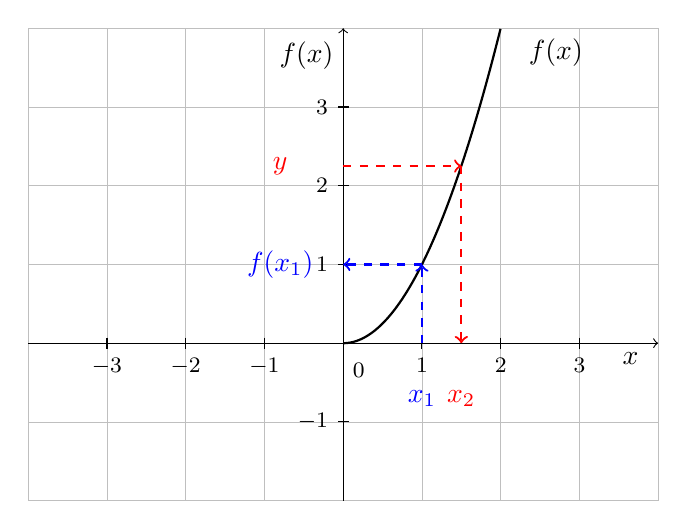
\begin{tikzpicture}
		
		% Gitternetzlinien
		\draw[xstep=1cm, ystep=1cm, very thin, color=lightgray] (-4,4) grid (4,-2);
		% x-Achse
		\draw[->] (-4,0) -- (4,0) node[below,xshift=-1em] {$x$}; 
		%Zahlen auf x-Achse
		\foreach \x in {-3,...,-1}
		\draw[shift={(\x,0)},color=black] (0pt,2pt) -- (0pt,-2pt) node[below] {\footnotesize $\x$};
		\foreach \x in {1,...,3}
		\draw[shift={(\x,0)},color=black] (0pt,2pt) -- (0pt,-2pt) node[below] {\footnotesize $\x$};
		% y-Achse 
		\draw[->] (0,-2) -- (0,4) node[left,yshift=-1em] {$f(x)$};%node[above left]
		%Zahlen auf y-Achse
		\foreach \y in {-1,...,-1}
		\draw[shift={(0,\y)},color=black] (2pt,0pt) -- (-2pt,0pt) node[left] {\footnotesize $\y$};
		\foreach \y in {1,...,3}
		\draw[shift={(0,\y)},color=black] (2pt,0pt) -- (-2pt,0pt) node[left] {\footnotesize $\y$};
		%Ursprung
		\draw[color=black] (0pt,-10pt) node[right] {\footnotesize $0$};
		
		
		
		\draw[thick,color=black] plot[samples=200, domain=0:2] 
		(\x,{\x*\x}) node[below, xshift=2em]{$f(x)$};
		
		\draw[->,color=blue,thick,dashed] (1,0) -- (1,1) ;
		\draw[->,color=blue,thick,dashed] (1,1) --  (0,1) ;
		
		\draw[color=blue,thick,dashed] (1,-0.7) node {$x_1$}  ;
		\draw[color=blue,thick,dashed] (-0.8,1) node {$f(x_1)$}  ;
		
		\draw[->,color=red,thick,dashed] (0,2.25) -- (1.5,2.25) ;
		\draw[->,color=red,thick,dashed] (1.5,2.25) --  (1.5,0) ;
		
		\draw[color=red,thick,dashed] (1.5,-0.7) node {$x_2$}  ;
		\draw[color=red,thick,dashed] (-0.8,2.25) node {$y$}  ;
		
	\end{tikzpicture}\\
\end{center}
Die Abbildung $f(x_1)$ geht von $x_1$ nach $f(x_1)$ und die Umkehrabildung von $y$ nach $x_2$.\vspace*{2mm}\\ 
Beispiel:\\

\begin{align*}
	f:&[0,\infty[\longmapsto[0,\infty[ \text{ mit } x\longmapsto x^2\\
	f^{-1}:&[0,\infty [\longmapsto[0,\infty[ \text{ mit }x\longmapsto \sqrt{x}\\ 
\end{align*} 
\begin{center}
	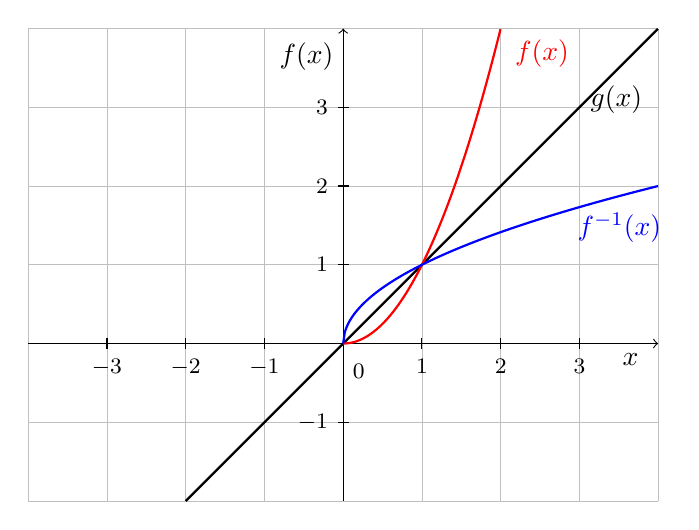
\begin{tikzpicture}
		% Gitternetzlinien
		\draw[xstep=1cm, ystep=1cm, very thin, color=lightgray] (-4,4) grid (4,-2);
		% x-Achse
		\draw[->] (-4,0) -- (4,0) node[below,xshift=-1em] {$x$}; 
		%Zahlen auf x-Achse
		\foreach \x in {-3,...,-1}
		\draw[shift={(\x,0)},color=black] (0pt,2pt) -- (0pt,-2pt) node[below] {\footnotesize $\x$};
		\foreach \x in {1,...,3}
		\draw[shift={(\x,0)},color=black] (0pt,2pt) -- (0pt,-2pt) node[below] {\footnotesize $\x$};
		% y-Achse 
		\draw[->] (0,-2) -- (0,4) node[left,yshift=-1em] {$f(x)$};%node[above left]
		%Zahlen auf y-Achse
		\foreach \y in {-1,...,-1}
		\draw[shift={(0,\y)},color=black] (2pt,0pt) -- (-2pt,0pt) node[left] {\footnotesize $\y$};
		\foreach \y in {1,...,3}
		\draw[shift={(0,\y)},color=black] (2pt,0pt) -- (-2pt,0pt) node[left] {\footnotesize $\y$};
		%Ursprung
		\draw[color=black] (0pt,-10pt) node[right] {\footnotesize $0$};
		\draw[thick,color=black] plot[samples=200, domain=-2:4] 
		(\x,{\x}) node[below, xshift=-1.5em,yshift=-1.7em]{$g(x)$};
		
		\draw[thick,color=red] plot[samples=200, domain=0:2] 
		(\x,{\x*\x}) node[below, xshift=1.5em]{$f(x)$};
		\draw[thick,color=blue] plot[samples=200, domain=0:4] 
		(\x,{sqrt(\x)}) node[below, xshift=-1.4em,yshift=-.6em]{$f^{-1}(x)$};
	\end{tikzpicture}\\
\end{center}
\textbf{Eigenschaften:}
\begin{quote}
	\textbullet $\;\; f^{-1}\circ f(x)=x=f\circ  f^{-1}$\\
	\textbullet $\;\; f(x)$ gespiegelt an der  Achse $f(x)=x$ ergibt die Umkehrfunktion $f^{-1}(x)$.
\end{quote}
Beispiel:\\
Sei $f(x)=x^2$ und 
$f^{-1}=\sqrt{x}$.\\
Bilde $f^{-1}\circ f$ und $f \circ f^{-1}$:
\begin{align*}
	f^{-1}(x)\circ f(x)=\sqrt{x^2}=x=(\sqrt{x})^2=f(x)\circ f^{-1}(x)\vspace*{4mm}\\
\end{align*}
\begin{tabular}[t]{lll}% l=linksbündig r=rechtsbündig
	Merke:&&\\
	& $f^{-1}$ & Umkehrfunktion \\
	& $\frac{1}{x^2}$ & Reziproke\\
	&$	 f^{-1}_{[0,\infty [}$& Urbild\\
\end{tabular} \\
\subsection{Aufgabe zur Umkehrabbildung Teil I}

%\textbf{Definition (Komposition):}\\
Sei $f(x)=x^2-2x$ gegeben.\\
\begin{tabular}[t]{lll}% l=linksbündig r=rechtsbündig
	(i) &Bestimme $\mathbb{D}_f$ max, so dass $f(x)$ umkehrbar ist.\\ 
	(ii)&Bestimme $f^{-1}(x)$  \\	
\end{tabular}\\ 
zu (i):
\begin{quote}
	$\mathbb{D}_f$ ist maximal, wenn  die Funktion bijektiv ist.\\
	$f(x)=x^2-2x$\\
	Nullstellen sind: $x_1=0$, $x_2=2$\\
	
	\begin{center}
		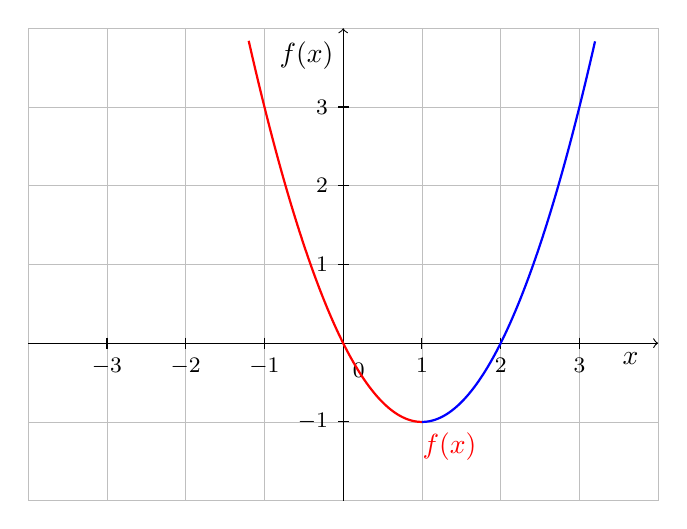
\begin{tikzpicture}
			
			% Gitternetzlinien
			\draw[xstep=1cm, ystep=1cm, very thin, color=lightgray] (-4,4) grid (4,-2);
			% x-Achse
			\draw[->] (-4,0) -- (4,0) node[below,xshift=-1em] {$x$}; 
			%Zahlen auf x-Achse
			\foreach \x in {-3,...,-1}
			\draw[shift={(\x,0)},color=black] (0pt,2pt) -- (0pt,-2pt) node[below] {\footnotesize $\x$};
			\foreach \x in {1,...,3}
			\draw[shift={(\x,0)},color=black] (0pt,2pt) -- (0pt,-2pt) node[below] {\footnotesize $\x$};
			% y-Achse 
			\draw[->] (0,-2) -- (0,4) node[left,yshift=-1em] {$f(x)$};%node[above left]
			%Zahlen auf y-Achse
			\foreach \y in {-1,...,-1}
			\draw[shift={(0,\y)},color=black] (2pt,0pt) -- (-2pt,0pt) node[left] {\footnotesize $\y$};
			\foreach \y in {1,...,3}
			\draw[shift={(0,\y)},color=black] (2pt,0pt) -- (-2pt,0pt) node[left] {\footnotesize $\y$};
			%Ursprung
			\draw[color=black] (0pt,-10pt) node[right] {\footnotesize $0$};
			
			
			
			\draw[thick,color=red] plot[samples=200, domain=-1.2:1] 
			(\x,{\x*\x-2*\x}) node[below, xshift=1em]{$f(x)$};
			
			\draw[thick,color=blue] plot[samples=200, domain=1:3.2] 
			(\x,{\x*\x-2*\x});
			
		\end{tikzpicture}\\
	\end{center}
	Offensichtlich ist $f:[1,\infty[\longmapsto [-1,\infty[$ in diesen Bereich bijektiv und ebenfalls ist $f:]-\infty,1]\longmapsto  [-1,\infty[$ bijektiv.\\
	Mengenmäßig ist die Menge; $]-\infty,1]$ größer als die Menge: $[1,\infty[$.
	Also ist $\mathbb{D}_f$ maximal mit:\\
	\begin{align*}
		f:]-\infty,1]\longmapsto  [-1,\infty[ \text{ mit }x\longmapsto x^2-2x\\
	\end{align*}
\end{quote}
\subsection{Aufgabe zur Umkehrabbildung Teil II}

zu (ii):
\begin{quote}
	Berechne $f^{-1}(x)$ mit der Funktion: $f:\;]-\infty,1]\longmapsto  [-1,\infty[ \text{ mit }x\longmapsto x^2-2x$\\
	Betrachte:\\
	$f(x)=y\Leftrightarrow x^2-2x=y\Leftrightarrow x^2-2x-y=0$\\
	Wie stellen die Gleichung auf $x$ um.\\
	\begin{align*}
		x^2-2x-y&=0\\
		x^2-2x+1-1&=y\\
		(x-1)^2&=1+y\\
		x-1&=\pm \sqrt{1+y}\\
		x_{1,2}&=1\pm \sqrt{1+y}\\
	\end{align*}
	Da der $\mathbb{D}_f=]-\infty,1]$ ist, muß die Wurzel negativ sein und die positive Wurzel spielt dadurch keine Rolle mehr.\\
	Also heißt die Umkehrfunktion $f^{-1}(y)=1-\sqrt{1+y}$\\
	Ob $f(x)$ oder $f(y)$ ist egal, kann man auch z nennen!\vspace*{2mm}\\
	Probe:\\
	es muß gelten für $f=x^2-2x$ und $f^{-1}=1-\sqrt{1+y}$:
	\begin{quote}
		$\bullet  \;\;f\circ f^{-1}$\\
		$\bullet \;\;f^{-1}\circ f$\\
		\begin{align*}
			f\circ f^{-1}(y)=f(1-\sqrt{1+y})&=(1-(\sqrt{1+y}))^2-2(1-\sqrt{1+y})\\
			&=1-2\sqrt{1+y}+1+y-2+2\sqrt{1+y}\\
			f\circ f^{-1}(y) &=y\\
			&\\
			f^{-1}(x)\circ f=f^{-1}(x^2-2x)&=1-\sqrt{x^2-2x-1}\\
			&=1-\sqrt{(1-x)}^2\\
			f^{-1}(x)\circ f&=1-(1-x)=x
		\end{align*}
		
		
	\end{quote}
	
\end{quote}
Die Umkehrfunktion lautet:\\
\begin{align*}
	f^{-1}:[-1,\infty[\longmapsto ]-\infty,1] \text{ mit }x\longmapsto 1-\sqrt{1+x}
\end{align*}
